\pagenumbering{arabic}
\setcounter{page}{11}
\chapter{Methodology}
An iterative and incremental software development approach, such as Agile methodology, can be adopted. Agile methodologies emphasize flexibility, collaboration,
and iterative development, which align well with the nature of the project and its
potential changes and refinements.\\

\section{Agile Methodology}
Agile development is a flexible and iterative approach to software development that prioritizes adaptability and collaboration. It emphasizes delivering small, incremental releases of a product with the goal of responding quickly to changing requirements and feedback. Agile methodologies are based on the Agile Manifesto, which values individuals and interactions, working solutions, customer collaboration, and responding to change over rigid processes and tools.\\
\begin{figure}[H]
    \centering
    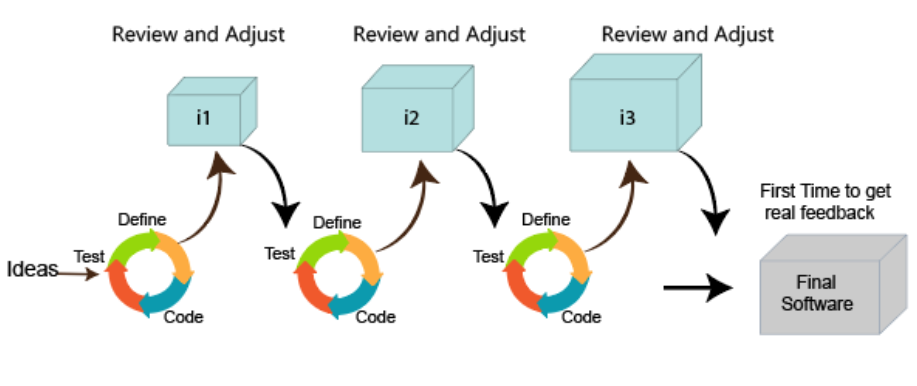
\includegraphics[width=1\textwidth]{img/agile.png}
    \caption{Agile methodology}
    \subcaption*{\textit{source: \textcolor{blue}{https://www.javatpoint.com/advantage-and-disadvantage-of-agile-methodology}}}
\end{figure}
The Agile development process is typically organized into iterations or sprints, each of which includes the following key steps:\\
\begin{itemize}

  \item \textbf{Requirements}:
        In Agile, requirements are expressed as user stories, which are short descriptions of a feature told from the perspective of the end user.
        Typically, the product owner collaborates with stakeholders to define and prioritize user stories, which in our case, are the objectives and highlights of the problem statement. These stories are added to the product backlog.

  \item \textbf{Design}:
        Design involves planning how the requirements will be implemented, considering the overall architecture, user interface, and other relevant aspects.
        During sprint planning, the development team discusses and plans how to address the problem statements and achieve the objectives. Design decisions are made collaboratively, and the team may create mockups or prototypes to visualize the solution.\\
  \item \textbf{Development}:
        This phase involves coding or implementing the solutions outlined in the design phase.
        Development work is carried out based on the tasks assigned to team members during the sprint planning. Continuous collaboration and communication are crucial to address any issues or changes that may arise.\\

  \item \textbf{Testing}:
        Testing is an integral part of Agile development and involves validating that the implemented features meet the specified requirements.
        Testing will be done parallely with development, creating test cases based on user stories and conducting various testing types (unit testing, integration testing, etc.) to ensure the quality of the code and output.\\

  \item \textbf{Deploy}:
        Deployment involves making the developed features available for use by end-users.
        The product increment is deployed to a staging or production environment. Continuous integration and deployment practices ensure that the latest changes are automatically integrated and deployed when ready.\\


  \item \textbf{Review}:
        At the end of each iteration, a review or demo is conducted to showcase the completed features to stakeholders.
        The team will participate in a review meeting to provide feedback, discuss any adjustments needed, and reprioritize the product backlog.\\

  \item \textbf{Launch}:
        The final step involves releasing the product increment to users. In our project, a web interface will be rolled at launch which will facilitate user interaction.
        Once all necessary adjustments are made based on feedback and the priorities based on objectives the product is officially launched. The cycle then repeats with a new iteration.\\
\end{itemize}

It's important to note that the design, development, testing, deployment, review, and launch steps occur iteratively and multiple times throughout the project. Agile development promotes continuous improvement and adaptation to changing requirements, allowing teams to deliver value to users more frequently and efficiently.\\



\pagebreak






